The temperatures in silicon detector systems are critically important to the performance of these systems. The leakage current shows a pronounced temperature dependence 
\begin{equation}
I\propto T_\text{S}^2e^{-T_\text{A}/T_\text{S}}
\end{equation}
where $T_\text{S}$ is the sensor temperature and $T_\text{A}\simeq7000$~K. Leakage currents can become particularly significant after irradiation of the silicon material. The heat generated by these leakage currents in the silicon sensor, together with the heat from front-end electronics components on the detector needs to be removed by cooling systems. Due to the strong growth of leakage power with temperature there is a critical temperature $T_\text{C}$, above which the heat cannot be removed quickly enough, and the detector becomes thermally unstable (`thermal runaway'). The capability of the cooling system in removing this heat is limited by the temperature of the local cold sink (typically the coolant temperature) and the thermal impedance of the heat path between the source (electronics and sensor) and the sink.

In addition, there can be aspects of the front-end electronics which are temperature-dependent. For example, in the strip system for the ATLAS phase~II upgrade (ref) there are two additional sources for temperature-dependent heat sources. The first is a radiation damage effect in the digital part of the readout-electronics (the ABC130 and HCC chips), which is manufactured in 130~nm technology by the xxx process (ref). This effect leads to a scaling of the digital power in the chip depending on the received dose rate (TID) and the temperature of the chip (ref). This has been first observed in the ATLAS IBL (ref). The other temperature dependence of the power generated by the front-end electronics stems from the temperature dependence of the converter chip (FEAST (ref)) used in the on-detector DC-DC converter system supplying power to the front-end electronics. 

Even before the limit of thermal stability is reached, knowledge of temperatures in silicon detector systems is important, as they define system parameters like power supply capacity and cable dimensions.

In principle the temperatures in the system for a given set of operational parameters (power density, thermal conductivities etc.) can be predicted by FEA to an accuracy which is given by the quality of the input parameters. However, this is a time-consuming process and can be prohibitively difficult if there is a large number of local heat sources depending non-linearly on the temperature. A simplification to this problem which allows for an analytical solution in the case of a simple heat source topology has been developed in \cite{Beck:2010zzd}. In this paper we develop this method further to include several temperature dependent non-linear heat sources in the front-end electronics. The resulting set of equations cannot be solved analytically any more, but with little effort using numerical problem solvers. This enables us to predict with some confidence the temperatures and power requirements in the ATLAS strip system throughout phase~II operation. The results from this prediction have been used throughout the project to consistently dimension the different systems (cooling, power, services etc.) also with some robustness due to the inclusion of a common set of safety factors. This method can be easily adapted to any other system after adjustment of the system specific geometries and parameters.

\subsection{The ATLAS strip system}
The strip system for the ATLAS phase II upgrade (ref TDR) consists of two parts: the barrel system comprised of four concentric cylindrical barrels and the two endcaps, which consist of six disks each.

In the barrel the detector modules are made of square sensors ($96.85\times 96.72$~mm$^2$) with a hybrid on top, which hosts the front-end chips (ABC* and HCC*), but also circuitry to convert the supply voltage of larger than 10~V to the chip voltage of 1.5~V. This circuitry is controlled by the FEAST chip. The modules are glued onto both sides of a composite sandwich which contains two parallel thin wall titanium cooling pipes embedded in carbon foam (Allcomp K9 - ref)  between two facesheets of UHM carbon fibre (3 layers of K13C2U/EX1515) with a co-cured Kapton/copper low-mass tape. A model of this geometry is shown in fig.~\ref{fig:barrelgeometry}. During final operation cooling will be achieved by evaporating CO$_2$ in the cooling pipes with a final target temperature of not higher than -35$^\circ$C anywhere on the stave. With the exception of the end region of the stave, where a side-mounted End-Of-Structure (EOS) card is located and the thermal path is degraded by the presence of electrically insulating ceramic pipe sections, the geometry of the stave is uniform along its length. 

\begin{figure}[ht]
\centering
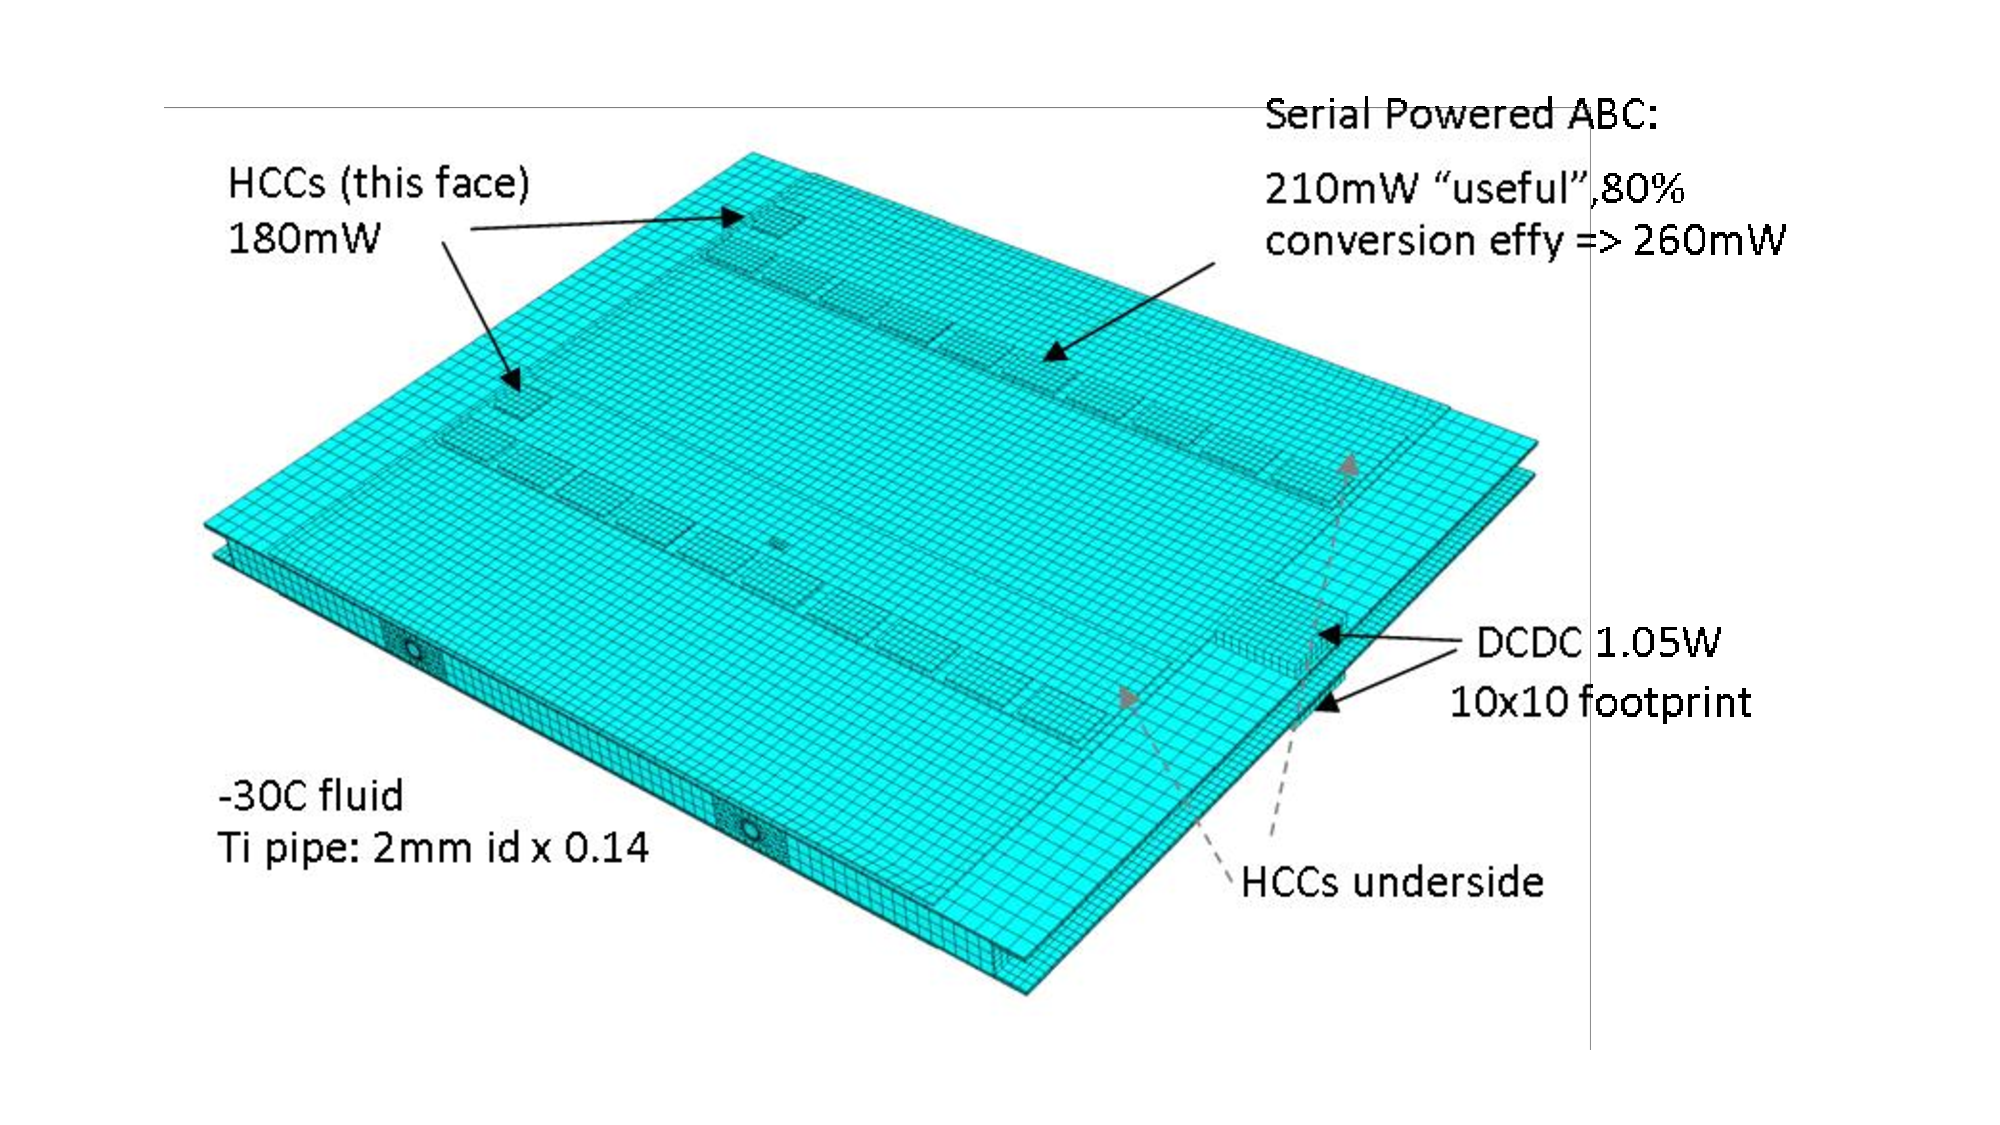
\includegraphics[width=0.4\linewidth]{figures/barrelmodule.pdf}
\caption{Barrel strip geometry}
\label{fig:barrelgeometry}
\end{figure}

The endcap detector consists of six disks, each containing 32 ``petals'' loaded on
both sides with six silicon modules (twelve total).
The endcap detector modules consist of six distinct designs located at increasing radius from the
beam pipe and labeled R0 through R5 (where ``R'' stands for ring). Each endcap module consists of one
or two irregularly-shaped silicon sensors, and a varying number of front-end chips on each module
(between 12 and 28 ABCs, and 2 to 4 HCCs). The EOS card is located adjacent to the R5 module, but the
cooling pipes (and not the electrical breaks) run directly underneath it, in contrast to the barrel EOS.
The remaining module and petal core design details are largely identical to the barrel module description above.
Fig.~\ref{fig:endcapgeometry} depicts the geometry of the endcap petal.

\begin{figure}[ht]
\centering
%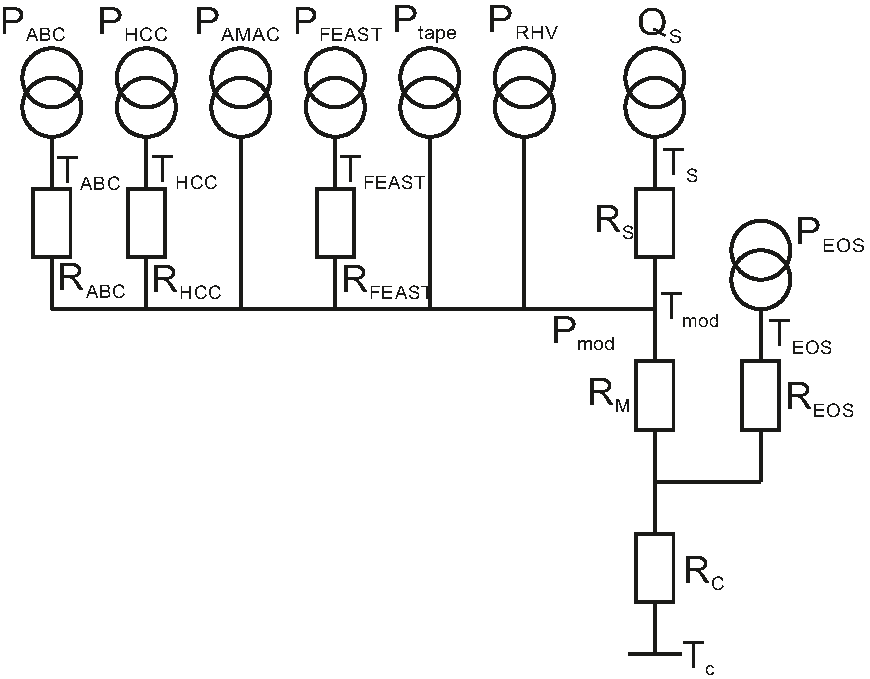
\includegraphics[width=0.6\linewidth]{figures/Thermalmodel.pdf}
\caption{Barrel strip geometry}
\label{fig:endcapgeometry}
\end{figure}

\subsection{Radiation environment}
